\chapter{Anhang}

\section{Verwendete Hilfsmittel}
In der Tabelle \ref{tab:tooling} sind die im Rahmen der Bearbeitung des Themas der \IthesisKindDE~verwendeten Werkzeuge und Hilfsmittel aufgelistet.

\begin{table}[h!] %TODO: ausfüllen
\caption{Verwendete Hilfsmittel und Werkzeuge}
\begin{tabular}{|l|l|}
\hline 
\rowcolor{lightgray} Tool & Verwendung \\
\hline
\LaTeX & Textsatz- und Layout-Werkzeug verwendet zur Erstellung dieses Dokuments \\
\hline
 & \\
\hline
\end{tabular}
\label{tab:tooling}
\end{table}

\section{Abbildungen}

\begin{figure}[htbp]
    \begin{center}
        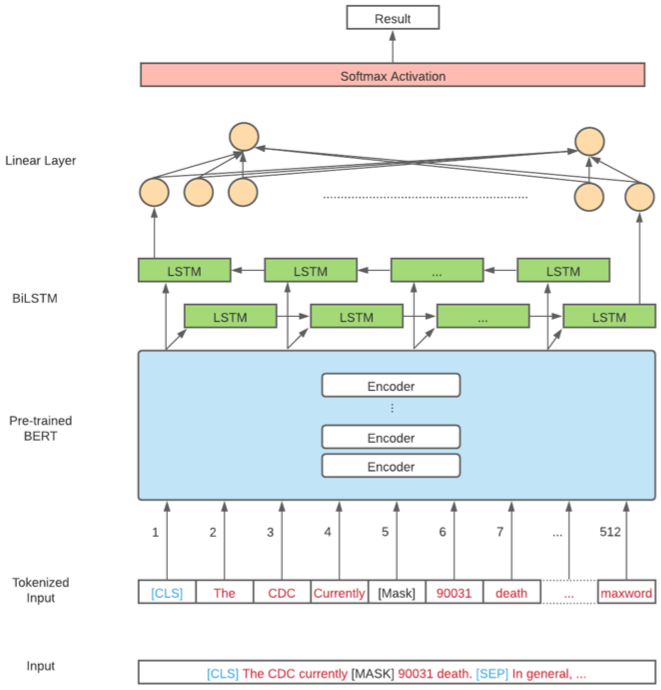
\includegraphics[scale=0.45]{static/bert_bilstm_architecture.png}
        \caption{\label{fig:bert_bilstm_architecture} Architektur des hybriden Modells \cite{wang2021covid19fakenewsdetection}}
    \end{center}
\end{figure}

\begin{figure}[htbp]
    \begin{center}
        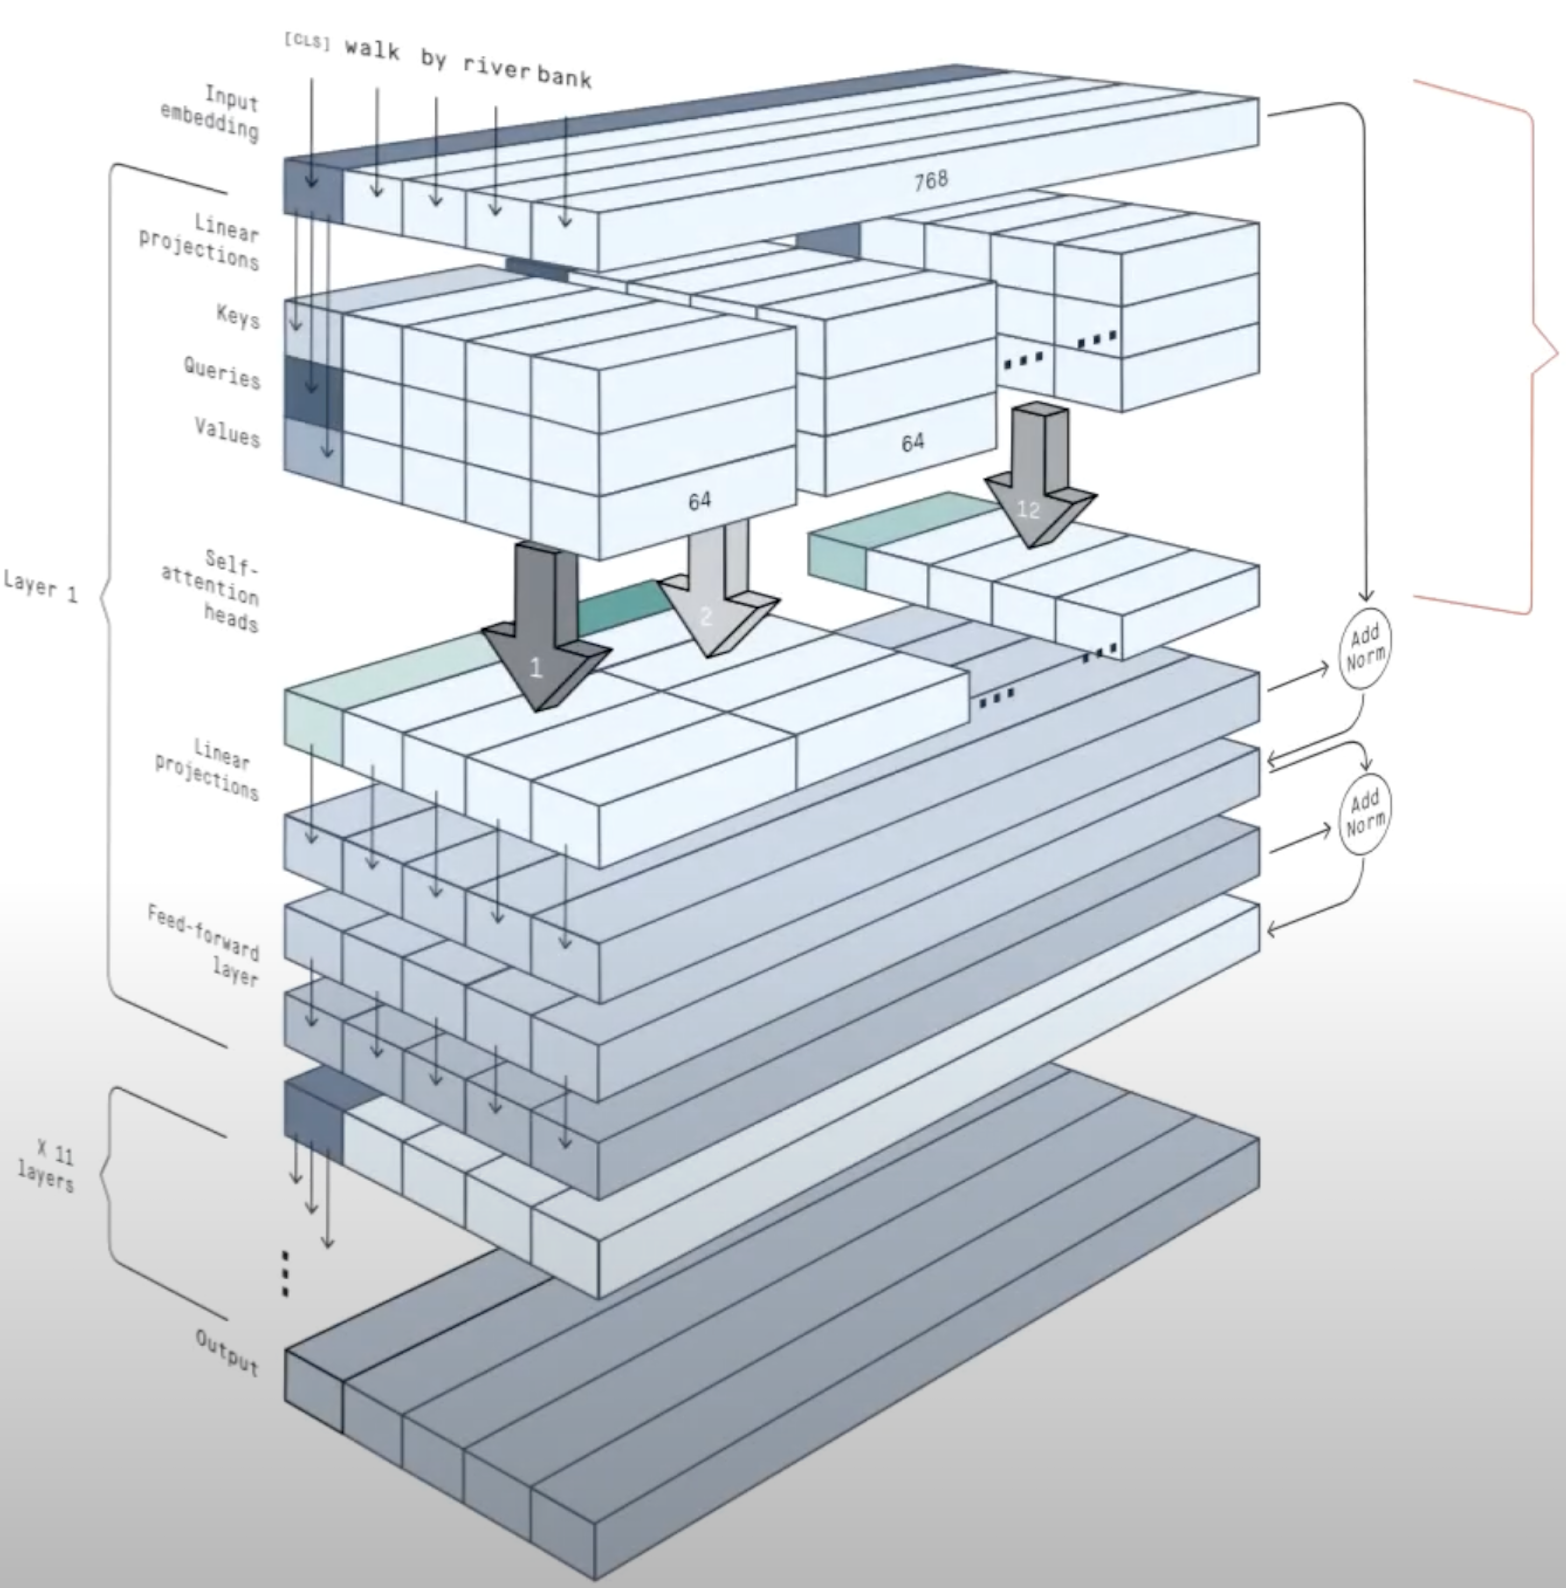
\includegraphics[scale=0.5]{static/BERT_visualization.png}
        \caption{\label{fig:BERT_visualization} Architektur des BERT Modells \cite{peltarion2020bert}}
    \end{center}
\end{figure}

\begin{figure}[htbp]
    \begin{center}
        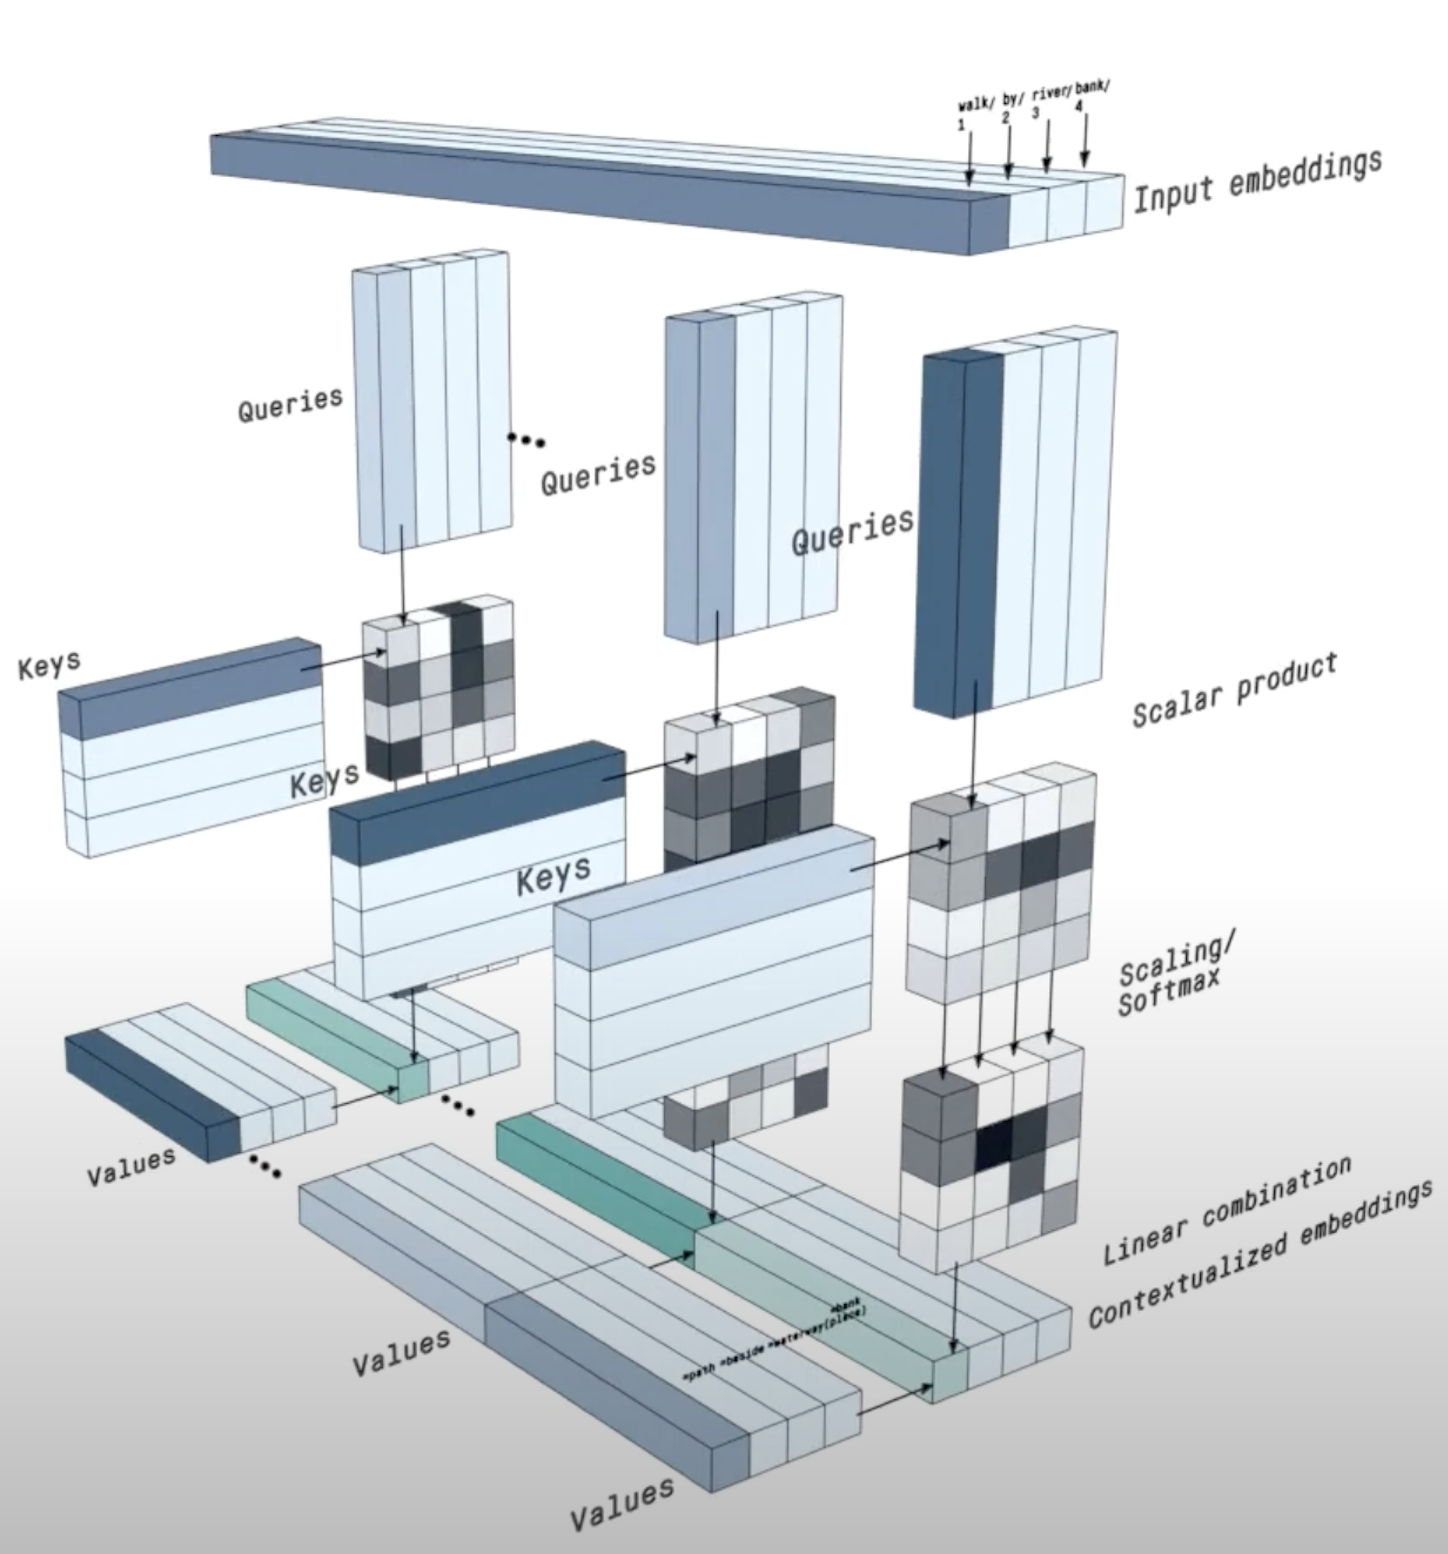
\includegraphics[scale=0.5]{static/multi-head_attention_visualization.png}
        \caption{\label{fig:multi_head_attention_visualization} Multi-Head Attention \cite{peltarion2020bert}}
    \end{center}
\end{figure}

\begin{figure}[htbp]
    \begin{center}
        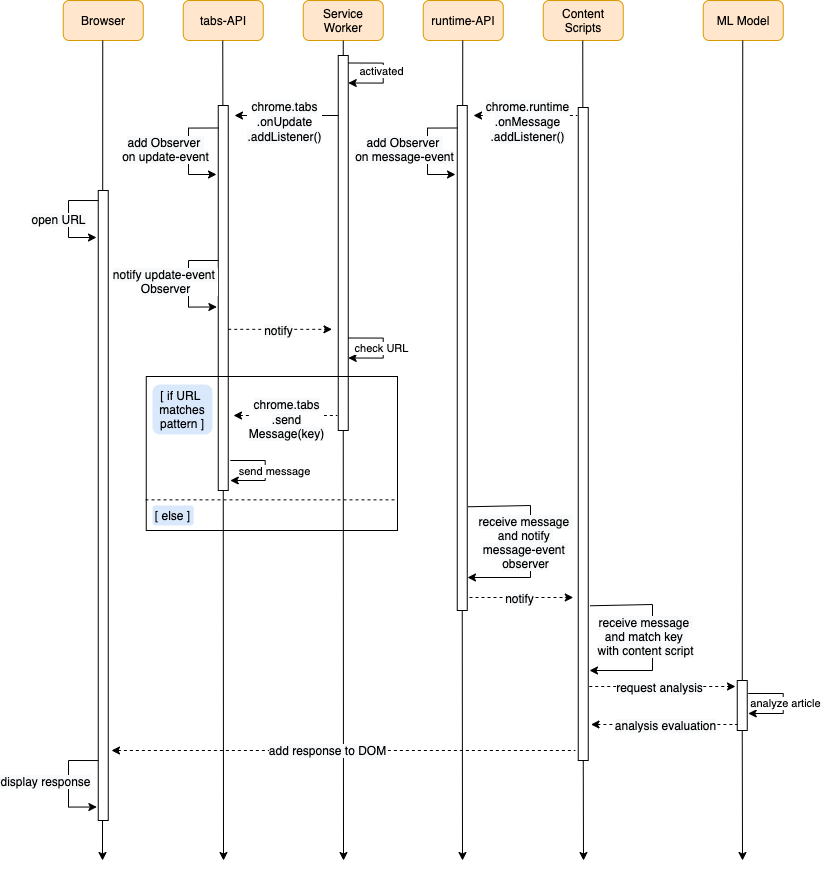
\includegraphics[scale=0.5]{diagrams/hauptkomponente_sequenzdiagramm.png}
        \caption{\label{fig:seq_hauptkomponente} Sequenzdiagramm Webagent}
    \end{center}
\end{figure}

\begin{figure}[htbp]
    \begin{center}
        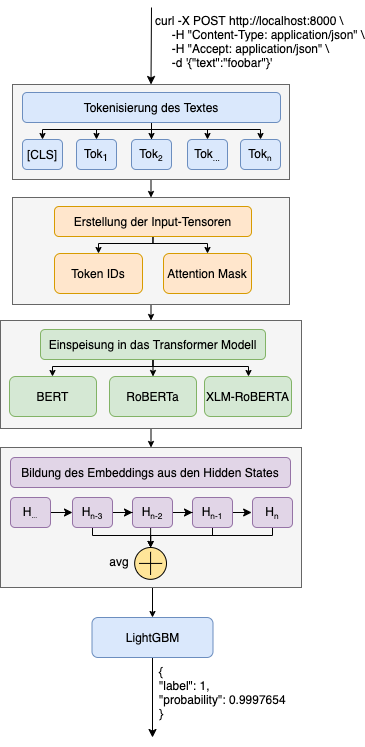
\includegraphics[scale=0.6]{diagrams/gesamtarchitektur.png}
        \caption{\label{fig:gesamtarchitektur} Gesamtarchitektur des Webservers}
    \end{center}
\end{figure}

\section{Tabellen}

\begin{table}[htbp]
    \centering
    \renewcommand{\arraystretch}{1.3}
    \begin{tabular}{|p{2.5cm}|p{2.5cm}|p{2.5cm}|p{2.5cm}|p{2.5cm}|}
        \hline
        \textbf{Kriterium} & \textbf{Chrome Extension} & \textbf{Userscript (Tampermonkey)} & \textbf{Proxy-Server} & \textbf{Scraper + Plattform} \\
        \hline
        DOM-Zugriff beim Nutzer & Ja & Ja & Nein & Nein \\
        \hline
        Einbindung auf \texttt{bild.de} direkt & Ja & Ja & Ja (indirekt) & Nein \\
        \hline
        Installation durch Nutzer & Mittel & Einfach & Nicht erforderlich & Nicht erforderlich\\
        \hline
        Komplexität der Umsetzung & Mittel & Gering & Hoch & Mittel \\
        \hline
        Wartbarkeit \& Updates & Gut & Gut & Aufwändig & Mittel \\
        \hline
        Performance beim Nutzer & Hoch & Hoch & Hoch & Hoch \\
        \hline
        Skalierbarkeit & Hoch & Eingeschränkt & Mittel & Hoch \\
        \hline
        Für öffentliche Verbreitung geeignet & Ja & Eingeschränkt & Eingeschränkt & Ja \\
        \hline
        API-Nutzung zur Fake-Erkennung & Ja & Ja & Ja & Ja \\
        \hline
        Entwickler-kontrolle über UI & Hoch & Mittel & Hoch & Mittel \\
        \hline
    \end{tabular}
    \caption{Vergleich möglicher Technologien für den Webagenten}
    \label{table:technischeAnsaetze}
\end{table} %TODO: ChatGPT


\begin{sidewaystable}[htbp]
    \centering
    \renewcommand{\arraystretch}{1.3}
    \begin{tabular}{|p{3.5cm}|p{2.8cm}|p{2.8cm}|p{2.8cm}|p{2.8cm}|p{2.8cm}|}
        \hline
        \textbf{Merkmal} & \textbf{BERT Base} & \textbf{RoBERTa\newline Base} & \textbf{RoBERTa Large} & \textbf{XLM-RoBERTa Base} & \textbf{XLM-RoBERTa Large} \\
        \hline
        \textbf{Hidden Size} & 768 & 768 & 1024 & 768 & 1024 \\
        \hline
        \textbf{Anzahl Layer} & 12 & 12 & 24 & 12 & 24 \\
        \hline
        \textbf{Anzahl Attention Heads} & 12 & 12 & 16 & 12 & 16 \\
        \hline
        \textbf{Vocab Size} & 30,522 & 50,265 & 50,265 & 250,002 & 250,002 \\
        \hline
        \textbf{Spezialisiert auf} & Masked LM & Masked LM & Masked LM & Multilinguales Masked LM & Multilinguales Masked LM \\
        \hline
        \textbf{Sprachumfang} & Englisch & Englisch & Englisch & Multilingual & Multilingual \\
        \hline
    \end{tabular}
\caption{Vergleich der verschiedenen BERT- und RoBERTa-Modelle}
\label{tab:bert_models}
\end{sidewaystable}

\begin{table}[htbp]
    \centering
    \renewcommand{\arraystretch}{1.3}
    \begin{tabular}{|p{3cm}|l|p{6cm}|}
        \hline
        \textbf{Parameter} & \textbf{Wert} & \textbf{Beschreibung} \\
        \hline
        Anzahl Trainingsepochen & \texttt{5} & Das gesamte Trainingsset wird fünfmal vollständig durchlaufen. \\
        \hline
        Batch-Größe & \texttt{32} & Anzahl der Beispiele, die gleichzeitig in einem Schritt verarbeitet werden. \\
        \hline
        Lernrate & \texttt{2e-5} & Bestimmt die Schrittweite der Modellaktualisierung bei jedem Optimierungsschritt. \\
        \hline
        Optimierungs-verfahren & \texttt{AdamW} & Variante des Adam-Optimierers mit Weight Decay, automatisch in Hugging Face integriert. \\
        \hline
        Gewichtsabnahme (Weight Decay) & \texttt{0.01} & Reguliert große Gewichtswerte, um Überanpassung zu vermeiden. \\
        \hline
        Lernraten-Scheduler & \texttt{Linear, 10\% Warmup} & Die Lernrate steigt linear an und wird anschließend schrittweise reduziert. \\
        \hline
        Kriterium für bestes Modell & \texttt{F1-Score} & Das Modell mit dem besten F1-Score auf den Validierungsdaten wird gespeichert. \\
        \hline
        Hardware-Beschleunigung & \texttt{fp16 aktiviert} & Angepasst auf A100 GPU zur Beschleunigung des Trainings. \\
        \hline
    \end{tabular}
    \caption{Überblick über die gewählten Hyperparameter der Transformer-Modelle}
    \label{tab:transformer-hyperparameter}
\end{table}


\begin{table}[htbp]
    \centering
    \renewcommand{\arraystretch}{1.1}
    \begin{tabular}{|p{3cm}|l|p{7cm}|}
        \hline
        \textbf{Parameter} & \textbf{Wert} & \textbf{Beschreibung} \\
        \hline
        Ziel (\texttt{objective}) & \texttt{binary} & Binäre Klassifikation (z.\,B. „echt“ oder „fake“). \\
        \hline
        Metrik (\texttt{metric}) & \texttt{binary\_logloss} & Verlustfunktion zur Bewertung der Modellgüte während des Trainings. \\
        \hline
        Boosting-Typ (\texttt{boosting\_type}) & \texttt{gbdt} & Verwendung von Gradient Boosted Decision Trees als Lernverfahren. \\
        \hline
        Prozessor-Kerne (\texttt{n\_jobs}) & \texttt{-1} & Nutzt alle verfügbaren CPU-Kerne für paralleles Training. \\
        \hline
        Lernrate (\texttt{learning\_rate}) & \texttt{0.0865} & Schrittweite beim Anpassen der Modellgewichte. \\
        \hline
        Anzahl Blätter (\texttt{num\_leaves}) & \texttt{63} & Maximale Anzahl von Blättern pro Entscheidungsbaum. \\
        \hline
        Maximale Tiefe (\texttt{max\_depth}) & \texttt{20} & Begrenzt die Tiefe der Bäume zur Kontrolle der Komplexität. \\
        \hline
        Min. Samples pro Blatt (\texttt{min\_child\_samples}) & \texttt{80} & Minimale Anzahl an Trainingsbeispielen pro Blatt. \\
        \hline
        Subsample-Rate (\texttt{subsample}) & \texttt{0.9818} & Anteil der Trainingsdaten, der zufällig pro Baum verwendet wird. \\
        \hline
        Merkmalsauswahl pro Baum (\texttt{colsample\_bytree}) & \texttt{0.9684} & Anteil der Merkmale, die pro Baum zufällig ausgewählt werden. \\
        \hline
        $L_1$-Regularisierung (\texttt{reg\_alpha}) & \texttt{0.2989} & Bestraft große Gewichtswerte zur Förderung einfacher Modelle. \\
        \hline
        $L_2$-Regularisierung (\texttt{reg\_lambda}) & \texttt{0.4609} & Stabilisiert das Modell durch Bestrafung großer Gewichtssummen. \\
        \hline
        Zufallsstart (\texttt{random\_state}) & \texttt{42} & Sichert Reproduzierbarkeit der Ergebnisse. \\
        \hline
        Anzahl Bäume (\texttt{n\_estimators}) & \texttt{2000} & Maximale Anzahl an Bäumen; Early Stopping begrenzt effektiv. \\
        \hline
    \end{tabular}
    \caption{Überblick über die gewählten Hyperparameter des LightGBM-Modells}
    \label{tab:lightgbm-hyperparameter}
\end{table}